\documentclass[12 pt]{article}
\usepackage{titling}
\usepackage[a4paper, margin = 1in]{geometry}
\usepackage{graphicx}
\usepackage{caption}
\usepackage{hyperref}
\usepackage{mathtools}
\usepackage{amsmath}
\usepackage{amssymb}
\usepackage{float}
\usepackage{longtable}
\usepackage{fancyhdr}
\usepackage[utf8]{inputenc}
\usepackage[T1]{fontenc}
\setlength{\parindent}{0ex}
\usepackage{setspace}
\usepackage{titlesec}
\usepackage{subcaption}

\setstretch{1.0}

\title{Literature Review – High Granularity Calorimeter at the CMS experiment at CERN}
\date{\today}
\author{Stephan Koenigstorfer \\ CID: 01049055} 

\pagestyle{fancy}
\fancyhf{}
\rhead{CID: 01049055}
\lhead{Stephan Koenigstorfer}
\chead{Msci Project}
\cfoot{ \textbf{\thepage}}

\begin{document}
	
	\maketitle
	\begin{figure}[H]
		\centering
		
\includegraphics[width=0.5\textwidth]{imperial_logo.png}
	\end{figure}
	
	\newpage
	
	\section*{Declaration of work}
		I confirm that this report was written by myself. I confirm that, except where stated otherwise through acknowledgements or references, the work presented within this report was carried out by my project partner and myself. Between the two of us the work was split evenly across all aspects. 
	\tableofcontents

	\newpage


	\begin{abstract}
	\end{abstract}

	\section{Introduction}
		The Large Hadron Collider (LHC) at CERN is currently being upgraded in order to explore new areas of physics. The general upgrade allows the LHC to explore higher energies, and the individual experiments are being upgraded to improve factors such as precision. This literature review is primarilarly concerned with the new High Granularity Calorimeter (HGCAL) at the CMS experiment. \\
		The new HGCAL needs is being built to im
	\section{Physics and Motivation}
		\subsection{LHC}
			The LHC experiment had a great first run, shedding light on the rare B$^0 \rightarrow \mu^+ \mu^-$ \cite{B0} decay as well as discovering the Higgs boson and investigating its properties. While the first of these discoveries placed tight constraints on any new physics theories beyond the standard model (SM) \cite{mot}, the latter was the discovery of a completely new type of boson. This allows for further testing of the SM, such as the shape of the Higgs field vacuum potential. Unfortunately, beyond 2019 it would take more than 10 years to half the statistical error with the current luminosity \cite{mot}.\\

			The high luminosity upgrade at the LHC will allow for the much improved investigation of the Higgs boson, specifically by drastically reducing the uncertainties on its coupling strengths to other bosons, fermions and to itself \cite{mot}.

			The above measurements will test the predictions of the SM, but equally, if not more important is finding evidence of physics beyond the SM. This will include testing for Supersymmetry (SUSY), weakly interacting massive particles (WIMPS) and other new physics \cite{mot}.
		\subsection{CMS \& HGCAL}
			This project is specifically concerned with the upgrade of the high granularity calorimeter (HGCAL) of the CMS experiment. Since the radiation exposure after the high luminosity upgrade will significantly exceed the specification of the original experiment, general performance can only be maintainted by adjusting the experiment to withstand the higher radiation dose \cite{TDR} \cite{mot}. This also provides the opportinuty to increase the resolution of the calorimeters \cite{PFAsInHCAL} \cite{calice}. 

			The upgrade will allow for 2 dimensional data readout, allowing better resolution and the application of Particle Flow algorithms (PFAs)(see section \ref{PFAs}. These in turn will greatly increase the resolution of individual particles' energies \cite{PFAsInHCAL}.
	\section{What to do for detection}
		\subsection{Electromagnetic and Hadronic showers}
			In order to measure the energy of a particle, it is necessary for it to deposit all this energy into the detector material. Fortunately, this process is facilitated by particle showers. The two important types are electromagnetic and hadronic showers \cite{notes13}. These both cause the creation of many particles at low energies (and momenta) out of a single particle of high energy. For the electronmagnetic case, this is due to a combination of two effects \cite{notes13}: 
			\begin{itemize}
				\item electron-positron pair production from $\gamma$s
				\item electrons undergoing bremsstrahlung
			\end{itemize}
			This happens on a characteristic lengscale $X_0$, called the radiation length, over which one interaction takes place. This shower continues for several lengthscales, until the average electron energy is sufficiently low such that it no longer radiates energy via photons but instead deposits all its energy into the detector material via Boethe-Bloch energy loss.\\
			Hadronic showers look fairly similar to electromagnetic showers. The excact mechanism is based on FILL IN THROUGH RESEARCH. \\
			Both electromagnetic and hadronic calorimeters make use of these showers in order to make an energy measurement. They do this by alternating dense material which induces the showers with detector materials which captures ionizing radiation \cite{notes13}. The typical length scale for the hadronic showers is much larger than the radiation length for electromagnetic showers, and is called the absorption length. In the detector, this means that if hadrons pass through an electromagnetic detector, they will barely interact. A diagram of a shower in such a detector can be seen in Figure \ref{particle_shower}.
			\begin{figure}[h]
				\centering
				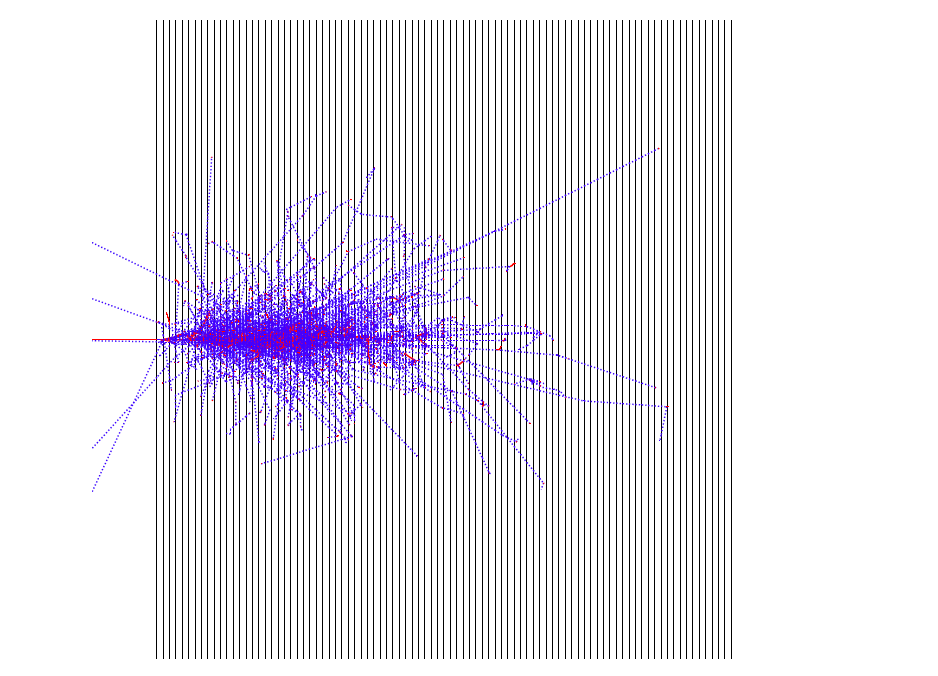
\includegraphics[width=0.9\textwidth]{particle_shower.png}
				\label{particle_shower}
				\caption{Figure showing an electromagnetic particle shower in a detector, as shown in \cite{notes13}.}
			\end{figure}
		\subsection{Particle detection}
			Particle detection occurs over several independent processes \cite{notes13}, as shown in Figure \ref{particle_detecion}. The first step involves identifying charged particles  tracking their paths, which is done with the use of magnetic fields. This yields a measurement of the momentum transverse to the magnetic field via the radius $R$ of the track. Since a magnetic field does no work, this is non-destructive of the later energy measurement. \\
			This is followed by an Electromagnetic Calorimeter, which absorbs electrons and photons based on an electron shower. Both particles leave similar tracks, but can be distinguished by the electron leaving a track in the earlier detector \cite{}. All other charged particles will leave only a small deposit. \\
			Next follows a hadronic calorimeter, which absorbs the protons, neutrons and K-longs. These are the hadrons stable enough to survive until they reach the detector. Other hadrons will decay (usually into these more stable hadrons \cite{}) before reaching the detector material. \\
			Finally, the only semi-stable particle left is the muon, which can then be seen in another magnetic tracking detector.
			\begin{figure}[h]
				\centering
				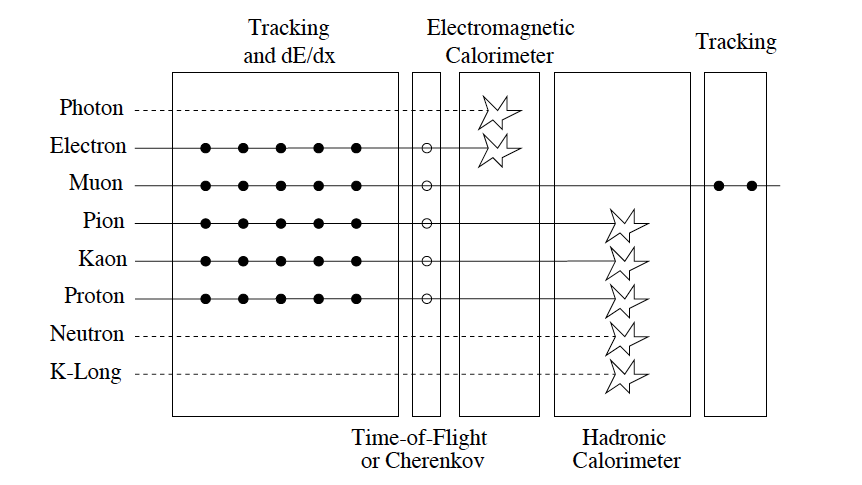
\includegraphics[width=0.9\textwidth]{particle_detection.png}
				\label{particle_detection}
				\caption{Figure showing different detection methods for different particles, as shown in \cite{notes13}.}
			\end{figure}
		\subsection{Minimum Ionizing Particles (MIPs)}
			A MIP is a useful way of classifying the minimum necessary precision of a detector. As a particle moves through a detector, it positions a certain amount of energy into the detector per unit distance ($\frac{dE}{dx}$), dependent on its momentum, the type of particle and the material it is moving through. At low momenta this ratio decreases with increasing momenta, however, due to relativity it starts to rise again at high momenta. This is called the "relativistic rise", and always causes a minimum in the plot of ($\frac{dE}{dx}$) vs $p$. A particle moving at this momentum is called a MIP, and is the most difficult to detect, since it deposits the least amount of energy into the detector material per distance. 

			The exact minimum points for different particles are very close together, and hence all particles are treated to bottom out at the same value, such that the MIP can be considered a universal parameter for a given detector material. 
	\section{The High Granularity Calorimeter}
		\subsection{Trigger system}
		\subsection{Hardware limitations}
		\subsection{HGCAL vs previous CMS Calorimeter}
	\section{What to get out}
		\subsection{Particle Flow Algorythms (PFAs)}\label{PFAs}
			PFAs provide a useful way to reduce the error on the parts of the calorimeter with less resolution \cite{PFAsInHCAL} \cite{PFAsDualReadout}. This is done by using the detector type with the lowest energy/momentum uncertainty for every particle type, and using the track observed to assign energy deposits in other detector types to the known particle. This is made significantly simpler in the proposed CMS upgrade, due to the high granularity \cite{PFAsInHCAL}.
		\subsection{L1 Trigger}
			The huge amounts of data produced in each BX cannot all be processed or stored. Therefore, a decision needs to be made for every BX on whether the physics was interesting enough to keep the data or not. The data is then stored in a "buffer", which allows for a processing time of 140BX, or 12.5$\mu s$ \cite{TDR}. Most of this time is needed for information transitions and off detector processes, thus only 3.5$\mu s$ are left for making this decision. This is known as the L1 trigger. 
			The required outcome is a Y/N decision. 
	\section{Conclusion}

	\bibliography{lit_rev}
	\bibliographystyle{ieeetr}{}

\end{document} 
